\section{Discussion}
\label{sec:discussion}

As can be seen, our approach only provides a noticeable improvement to the performance of Cassandra when multiple nodes in the cluster are heavily loaded. This is not what we initially imagined our results would be. One of our intuitions is that the performance decreases because the resource usage formula does not accurately reflect what the time to execute a query will be. To confirm this intuition we performed an experiment that compared the resource usage to the query execution time in a Cassandra instance.

In the remainder of this section we will provide what we feel will be a more accurate resource usage formula for distributed databases, as well as discuss several limitations that may also have affected our work.

\subsection{Re-examining the Resource Usage formula}
\label{sec:examineResUse}

\begin{figure}[t]
\centering
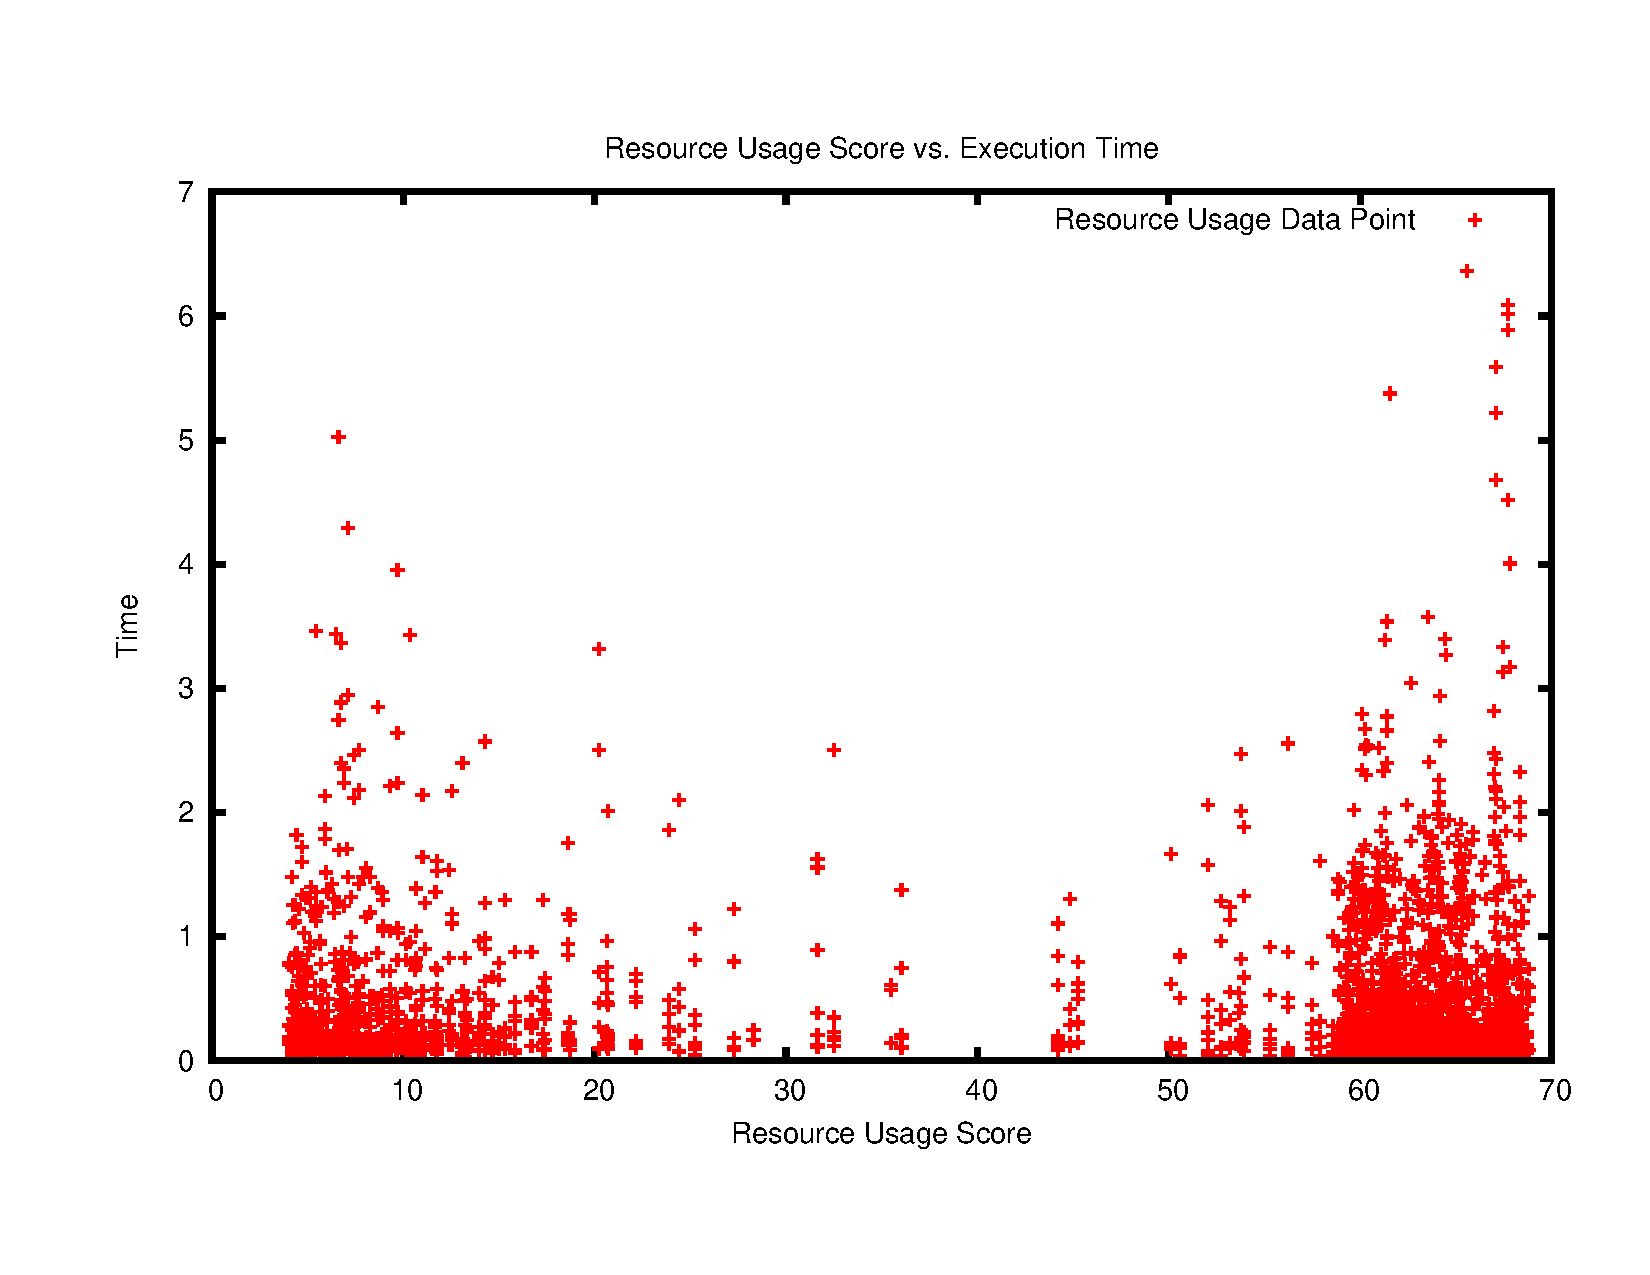
\includegraphics[scale=0.3]{images/ResUse.pdf}
\vspace{-15pt}
\caption{The experimental results comparing the resource usage score to the query execution time.}
\label{fig:resourceUsageFig}
\end{figure}

To examine how representative the resource usage score is, we have performed an experiment that compares resource usage to query execution time. The setup for the resource usage experiments is different than the setup for the primary experiments. This experiment was performed on a single Cassandra instance on a single machine with a 4-core 2.6Ghz processor and 8GB of memory. The server also contained a solid-state drive instead of the hard disk drive used in the servers in the cluster. The settings for YCSB and Cassandra were identical, except that the replication factor was set to \textit{one}.

The CPU and memory usage was recorded every 250ms, and the query execution time was recorded for each query. The queries that executed in that 250ms window had their execution time averaged. The CPU usage and memory usage were used to calculate the resource usage score of the server for each 250ms interval. The results were gathered over a 300 second interval using 10 parallel YCSB clients. Given our previous results showing that even 1000 parallel clients did not heavily load the node servers we do not believe that the results would be any different for a number of parallel clients greater than 10.

The results from the experiment are shown in Figure~\ref{fig:resourceUsageFig}. There appears to be little correlation between the resource usage score and the query execution time. When the resource usage score is higher, there are slightly more outliers that require a longer execution time, but in most cases the execution time seems to be independent of the resource usage. In addition, the resource usage scores tend to either be very low or very high. While this experiment was running, we also periodically loaded the server with other work. This resulted in a higher resource usage score, but not in a higher query execution time.

This experiment indicates that the current formula is not ideal for determining the resource usage of the server. However, we believe that the method could still work if the formula was changed to reflect how some variables affect the query execution time much more.  Additional variables can also be added to the formula. For example, one of the primary bottlenecks in any database system is the hard disk, and we did not consider any variables related to the disk (e.g., disk access throughput).

Something to note is that the heap memory of the Cassandra instance rarely exceeded 1GB, meaning that the memory usage score has little effect during the normal experiments. This means that very little data is being cached, which increases the importance of measuring the disk load.

\subsection{The New Resource Usage Formula}
\label{sec:usageFormula}
As Section~\ref{sec:examineResUse} shows, the resource usage score is not ideal. We have some ideas on creating a better resource usage formula. For reference, the current resource usage formula is:

\begin{center}
$ResourceUsage = \frac{1}{1-CPU} \times \frac{1}{1-Memory}$
\end{center}

Instead we propose a new equation that we feel may be more representative of the machine condition and should work better as a reference for assigning jobs:

\begin{center}
$ResourceUsage = \frac{1}{1-CPU} \times j\left ( \frac{1}{1-Memory} \right ) \times k\left ( \frac{1}{1-Disk} \right ) \times \frac{1}{1-Distance}$
\end{center}

As can be seen, the \textit{CPU usage} and \textit{Memory usage} are still in the equation. We have added parameters for \textit{Disk} usage, \textit{Distance} (network overhead) and two scaling parameters:

\begin{itemize}
\item{Disk} \\
\textit{Disk} refers to the hard disk performance of the machine. We feel this value should be related to values such as the average disk access time and data transfer rate. It will also be related to the disk usage by all programs on the machine. The slower the disk is by nature, and the busier the disk is being used by the programs, the higher the value of \textit{Disk} will be. 
\item{Distance} \\
\textit{Distance} is referring to the distance between the node servers and the condition of the network. This value will be determined by both the physical network ability, like the total available bandwidth; and the network conditions, like current network usage. This parameter is very important in affecting the execution time when dealing with multiple datacenters.
\item{Parameters \textit{k,j}} \\
The different server performance parameters have a different magnitude of effect on the query execution time. For example, from what we observed during the experiments, memory usage has little influence on the query execution time while \textit{disk usage} affects the execution time significantly. This importance level is adjusted by the constant coefficients \textit{j} and \textit{k} in the equations. \textit{Memory} is less important so \textit{j} should probably be less than 1 and \textit{disk} is very important so \textit{k} is probably bigger than 1. The exact value of these parameters would need to be determined with further testing.
\end{itemize}

This equation is just a representation of our idea and isn't necessarily accurate. More experiments are needed to confirm that this equation leads to better performance. 

\subsection{Limitations}
Our experiment is limited by the following factors:

\paragraph{Limited test environment}
As mentioned earlier, we only have ten servers in our experiment which limits the replica allocation. The distance between the servers is also extremely short, such that latency was never as issue. In reality, there are an average of 100,000 servers in a data center~\cite{Guo:2010:SDC:1921168.1921188}, and replication and backup processes may occur between data centers~\cite{F5-Accelerate}. In addition, normally every one mile in distance will add 8.2 microseconds latency to the performance, and this does not even consider package drop, switch delay, and link size~\cite{Cisco-Latency}.
 
\paragraph{Simplistic workload}
The queries, which we use to test our system, are simple. Even though we implemented our algorithm on the most time consuming queries in Cassandra, CPU and memory consumption was rare. This is because we are using a key-value database where the operations simple. This seems to partially account for why our approach does not introduce any performance improvement to the original query assignment system.
 
\paragraph{Unable to congest the network manually}
Network congestion occurs when a link is carrying data which is greater than the capacity of the network. This causes queuing delay, packet loss, and a high chance of failure~\cite{103559}. However, we do not have this issue in our experiment because our severs are located in close proximity and the network is never congested. This eliminates the chance to test our system under this situation.

\subsection{Future Work}
As mentioned above, we want to validate our proposed new resource usage formula (see Section~\ref{sec:usageFormula}) by running experiments on it. After determining a more accurate representation for the resource usage of a machine, the experiments could be redone to see if it leads to better performance. At the same time, we should continue to reduce the overhead of the query assignment algorithm as overhead is one of the key factors that affect the performance of the database.

We would also like to test our new algorithm on other key-value databases (e.g., HBase) and other types of databases (e.g., distributed relational databases). In the case of relational databases, more complex queries could be used to see how the complexity of queries affect the performance.

\section{Conclusion}
\label{sec:conclusion}
In this paper, we have examined the relationship between the resource usage of a machine and the time to execute a query. We have implemented a query assignment algorithm in Cassandra that takes into account the resource usage when assigning queries to nodes in the database cluster. We have found that although our method performs worse on average, there are certain cases where it provides superior performance to the default method in Cassandra. 

We have also found that CPU and memory usage tend to have a small impact on the query execution time. We believe that disk usage and network bandwidth are the more important factors. Based on our findings, we have proposed a new formula to represent the machine computing capacity more accurately. However, to draw any further conclusions about the proposed method, more study is required.
